\chapter{Orchestrated Objective Reduction (Orch-OR) Theory}
\label{ch:orch-or}

\begin{nontechnical}
\textbf{Orch-OR is a controversial theory claiming consciousness comes from quantum physics happening in tiny tubes inside brain cells---like your thoughts are quantum computers running in microscopic scaffolding!}

\textbf{The wild idea}: - \textbf{Normal view}: Brain = electrical
signals between neurons = consciousness - \textbf{Orch-OR view}: Brain =
quantum superpositions in microtubules = consciousness - \textbf{Why
controversial}: Most scientists think it\textquotesingle s impossible
(brain too warm/wet for quantum effects)

\textbf{The two scientists}:

\textbf{1. Roger Penrose} (Nobel Prize-winning physicist): -
``Consciousness can\textquotesingle t be explained by normal computing''
- ``Quantum mechanics must collapse in an objective way
(gravity-related)'' - ``This creates conscious moments''

\textbf{2. Stuart Hameroff} (anesthesiologist): - ``Microtubules
(protein tubes in neurons) are quantum computers'' - ``Anesthesia works
by disrupting quantum effects in microtubules'' - ``This explains why
diverse drugs all cause unconsciousness''

\textbf{Simple analogy - Orchestra}:
\begin{itemize}
\item \textbf{Neurons}: Like musicians in orchestra (play notes)
\item \textbf{Microtubules}: Like the conductor's baton oscillations (quantum superpositions)
\item \textbf{Orch-OR}: Baton collapses $\rightarrow$ orchestra plays note $\rightarrow$ conscious moment!
\item Happens $\sim$40 times/second $\rightarrow$ stream of consciousness
\end{itemize}

\textbf{What are microtubules?} - Tiny hollow tubes made of proteins
(tubulin) - In every cell (not just neurons) - Normally: Act as cell
skeleton, transport highways - Orch-OR claim: Also quantum computers for
consciousness!

\textbf{The big problem - ``Too warm, too wet''}:
\begin{itemize}
\item Quantum effects usually need: Cold (near absolute zero), isolated, vacuum
\item Brain is: 37°C, wet, chaotic, full of molecules
\item \textbf{Objection}: ``Quantum coherence would die in $10^{-13}$ seconds---way too fast!''
\item \textbf{Response}: ``Quantum biology shows nature is cleverer---see photosynthesis, bird navigation''
\end{itemize}

\textbf{Evidence FOR Orch-OR}: - \textbf{THz resonances found}:
Microtubules vibrate at specific frequencies (lab experiments) -
\textbf{Anesthetics bind to tubulin}: Explains why they cause
unconsciousness - \textbf{Quantum biology exists}: Photosynthesis, bird
magnetoreception use quantum effects - \textbf{Meyer-Overton rule}:
Anesthetic potency correlates with microtubule binding

\textbf{Evidence AGAINST Orch-OR}: - \textbf{Decoherence calculations}:
Quantum states should die too fast - \textbf{No direct proof}: Never
measured quantum superposition in living neurons - \textbf{Classical
explanation works}: Regular neural networks explain most consciousness -
\textbf{Mainstream skepticism}: Most neuroscientists/physicists
don\textquotesingle t buy it

\textbf{Why it matters for this project (Chimera/AID)}:

\textbf{IF Orch-OR is true}, then: 1. Microtubules have \textbf{resonant
frequencies} (0.2-2+ THz) 2. External \textbf{THz radiation} could
couple to these vibrations 3. Could \textbf{modulate} quantum states in
microtubules 4. Could \textbf{alter} conscious experience (inject
information?) 5. This is the \textbf{theoretical basis} for the AID
protocol speculation

\textbf{The experiment}: - Scientists (Bandyopadhyay et al.) put
microtubules in lab - Hit them with THz radiation - Found:
\textbf{Resonances at specific frequencies!} - Interpretation:
Microtubules can oscillate coherently - Question: Does this happen in
living brains?

\textbf{Real-world test - Anesthesia}:
\begin{itemize}
\item Put patient under with gas anesthetic
\item Orch-OR predicts: Gas binds to microtubules $\rightarrow$ quantum effects stop $\rightarrow$ consciousness off
\item Standard view: Gas affects GABA receptors $\rightarrow$ neurons quiet $\rightarrow$ consciousness off
\item Both might be partly true!
\end{itemize}

\textbf{The consciousness question}: - \textbf{Hard problem}: Why do we
have subjective experience? - \textbf{Orch-OR answer}: Quantum collapse
creates ``aha!'' moment - \textbf{Classical answer}: Emergent property
of complex neural networks - \textbf{Truth}: Nobody knows yet!

\textbf{Current status (2025)}: - \textbf{Mainstream}: ``Probably wrong,
but interesting'' - \textbf{Hameroff/Penrose}: ``Still viable, needs
better experiments'' - \textbf{Quantum biologists}: ``Less crazy than we
thought 10 years ago'' - \textbf{Verdict}: \textbf{Unproven but not
impossible}

\textbf{Why you should care}: - If true: Opens door to THz
neuromodulation (the AID protocol idea) - If false: AID protocol has no
theoretical basis - Either way: Pushes boundaries of what biology can do

\textbf{The philosophical bombshell}:
\begin{itemize}
\item If consciousness is quantum $\rightarrow$ Classical AI can't be conscious!
\item Need quantum computers + biological architecture
\item Free will might be quantum indeterminacy
\item Deep implications for mind/body problem
\end{itemize}

\textbf{Fun fact}: Roger Penrose won the Nobel Prize in Physics (2020) for work on black holes---NOT for Orch-OR! Most physicists respect his black hole work but are skeptical of his consciousness theories. It's a reminder that even brilliant scientists can have controversial ideas!
\end{nontechnical}

\begin{calloutbox}{Historical Note}
Sir Roger Penrose received the 2020 Nobel Prize in Physics for groundbreaking work on black hole formation---\textbf{not} for Orch-OR theory. The scientific community highly respects his contributions to general relativity while remaining skeptical of his consciousness hypotheses. This illustrates that even towering intellects can pursue controversial ideas outside mainstream consensus.
\end{calloutbox}

\section{Overview}

\textbf{Orchestrated Objective Reduction (Orch-OR)} is a controversial theory of consciousness proposed by physicist \textbf{Sir Roger Penrose} and anesthesiologist \textbf{Stuart Hameroff} in the mid-1990s.

\begin{keyconcept}
Orch-OR proposes that \textbf{consciousness arises from quantum computations in neuronal microtubules}, with orchestrated collapse of quantum superpositions (objective reduction) generating moments of conscious awareness at approximately 40~Hz (gamma rhythm).
\end{keyconcept}

This theory bridges quantum mechanics, neuroscience, and philosophy of mind, suggesting that consciousness is fundamentally quantum-mechanical rather than purely classical computational.



\section{Overview}

\textbf{Orchestrated Objective Reduction (Orch-OR)} is a controversial theory of consciousness proposed by physicist \textbf{Sir Roger Penrose} and anesthesiologist \textbf{Stuart Hameroff} in the mid-1990s.

\begin{keyconcept}
Orch-OR proposes that \textbf{consciousness emerges from quantum computations in neuronal microtubules}, with orchestrated collapse of quantum superpositions (objective reduction) generating discrete moments of conscious awareness at approximately 40~Hz.
\end{keyconcept}

\section{Theoretical Foundation}

\subsection{Penrose's Objective Reduction (OR)}

\textbf{Sir Roger Penrose} (Oxford physicist, Nobel laureate 2020) proposed fundamental modifications to quantum mechanics:

\begin{itemize}
\item \textbf{Quantum incompleteness:} Standard quantum theory cannot account for consciousness
\item \textbf{Objective collapse:} Wave function reduction is a physical process, not merely observer-dependent
\item \textbf{Gravitational mechanism:} Spacetime curvature drives superposition collapse
\item \textbf{Planck-scale threshold:} Collapse occurs when gravitational self-energy reaches quantum limit
\end{itemize}

\textbf{Mathematical criterion for objective reduction:}
\begin{equation}
\label{eq:or-criterion}
E \cdot \tau \approx \hbar
\end{equation}
where:
\begin{itemize}
\item $E$ = gravitational self-energy of quantum superposition (J)
\item $\tau$ = collapse timescale (s)
\item $\hbar = 1.055 \times 10^{-34}$~J$\cdot$s = reduced Planck constant
\end{itemize}

\textbf{Key principle:} Larger mass superpositions generate greater spacetime curvature differences, triggering faster objective collapse. This provides an intrinsic timescale for wave function reduction independent of measurement.

\subsection{Hameroff's Microtubule Computing}

\textbf{Stuart Hameroff} (University of Arizona anesthesiologist) provided the biological substrate:

\begin{itemize}
\item \textbf{Quantum computation substrate:} Microtubules serve as biological quantum processors
\item \textbf{Tubulin qubits:} Electron configurations in tubulin dimers encode quantum information
\item \textbf{Orchestration mechanism:} Microtubule-associated proteins (MAPs) coordinate quantum state evolution
\item \textbf{Anesthesia explanation:} General anesthetics bind to tubulin hydrophobic pockets, disrupting quantum coherence
\end{itemize}

\subsection{Integrated Orch-OR Framework}

\textbf{Synthesis} (Penrose $+$ Hameroff):

\begin{enumerate}
\item \textbf{Superposition formation:} Quantum states develop across microtubule tubulin networks
\item \textbf{Orchestrated evolution:} MAPs and cellular environment guide quantum state dynamics
\item \textbf{Objective reduction:} Gravitational self-energy threshold triggers collapse (Eq.~\ref{eq:or-criterion})
\item \textbf{Conscious moment:} OR event generates discrete instance of awareness
\item \textbf{Repetition:} Process cycles at $\sim$40~Hz, producing continuous conscious experience
\end{enumerate}

\textbf{Neural processing cycle:}

\begin{center}
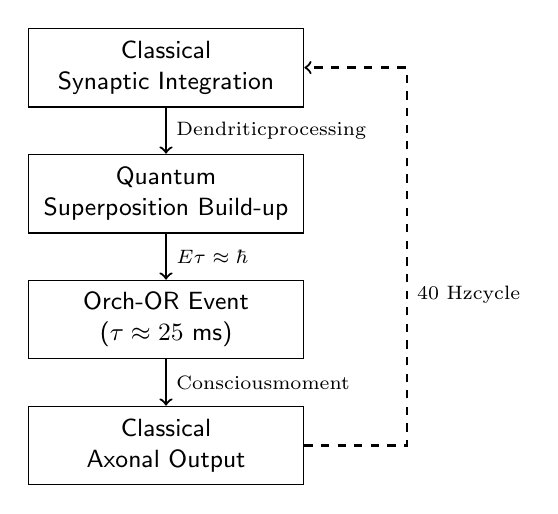
\begin{tikzpicture}[
  block/.style={rectangle, draw, minimum width=3.5cm, minimum height=1cm, font=\sffamily\small, align=center},
  node distance=1.6cm,
  font=\small
]
\node[block] (input) {Classical\\Synaptic Integration};
\node[block, below of=input] (quantum) {Quantum\\Superposition Build-up};
\node[block, below of=quantum] (orchor) {Orch-OR Event\\($\tau \approx 25$~ms)};
\node[block, below of=orchor] (output) {Classical\\Axonal Output};

\draw[->,thick] (input) -- node[right,font=\scriptsize,pos=0.5] {Dendritic\\processing} (quantum);
\draw[->,thick] (quantum) -- node[right,font=\scriptsize,pos=0.5] {$E\tau \approx \hbar$} (orchor);
\draw[->,thick] (orchor) -- node[right,font=\scriptsize,pos=0.5] {Conscious\\moment} (output);
\draw[->,thick,dashed] (output.east) -- ++(1.3,0) |- node[pos=0.2,right,font=\scriptsize] {40~Hz\\cycle} (input.east);
\end{tikzpicture}
\end{center}

\section{Microtubule Structure and Function}

\subsection{Structural Anatomy}

\textbf{Microtubules} are hollow cylindrical protein polymers with the following characteristics:

\begin{center}
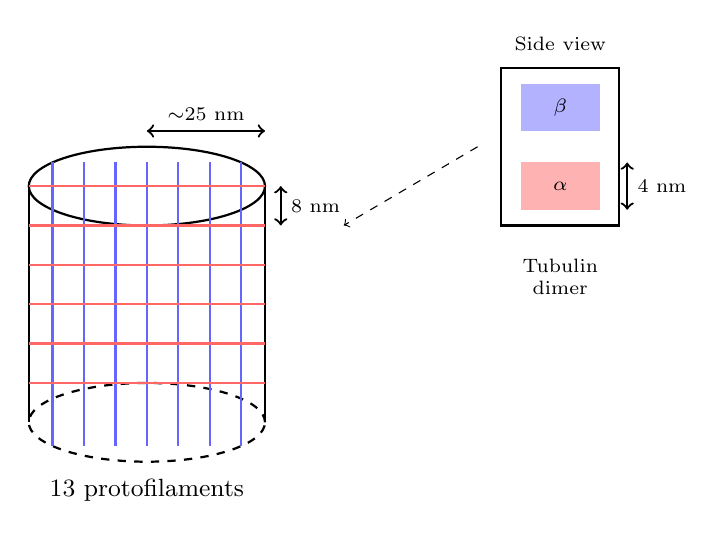
\begin{tikzpicture}[scale=1.0]
% Draw cylinder representation
\draw[thick] (0,0) ellipse (1.5 and 0.5);
\draw[thick] (-1.5,0) -- (-1.5,-3);
\draw[thick] (1.5,0) -- (1.5,-3);
\draw[thick,dashed] (0,-3) ellipse (1.5 and 0.5);

% Protofilaments (8 visible ones for clarity)
\foreach \x in {-1.2,-0.8,-0.4,0,0.4,0.8,1.2} {
  \draw[blue!60,thick] (\x,0.3) -- (\x,-3.3);
}

% Tubulin dimers
\foreach \y in {0,-0.5,-1.0,-1.5,-2.0,-2.5} {
  \draw[red!60,thick] (-1.5,\y) -- (1.5,\y);
}

% Labels
\draw[<->,thick] (1.7,0) -- (1.7,-0.5) node[midway,right,font=\scriptsize] {8 nm};
\draw[<->,thick] (0,0.7) -- (1.5,0.7) node[midway,above,font=\scriptsize] {$\sim$25 nm};
\node[below,font=\small] at (0,-3.6) {13 protofilaments};

% Side view detail - repositioned to avoid overlap
\begin{scope}[xshift=4.5cm, yshift=-0.5cm]
  \node[above,font=\scriptsize] at (0.75,2.1) {Side view};
  \draw[thick] (0,0) rectangle (1.5,2);
  \fill[red!30] (0.25,0.2) rectangle (1.25,0.8);
  \fill[blue!30] (0.25,1.2) rectangle (1.25,1.8);
  \node[font=\scriptsize] at (0.75,0.5) {$\alpha$};
  \node[font=\scriptsize] at (0.75,1.5) {$\beta$};
  \draw[<->,thick] (1.6,0.2) -- (1.6,0.8) node[midway,right,font=\scriptsize] {4 nm};
  \node[below,font=\scriptsize,align=center] at (0.75,-0.3) {Tubulin\\dimer};
  
  % Connection line to main diagram
  \draw[->,dashed,thin] (-0.3,1) -- (-2,0);
\end{scope}
\end{tikzpicture}
\end{center}

\textbf{Structural parameters:}
\begin{itemize}
\item \textbf{Outer diameter:} $\sim$25~nm
\item \textbf{Inner diameter:} $\sim$15~nm (hollow core)
\item \textbf{Length:} Micrometers to millimeters (dynamic)
\item \textbf{Composition:} $\alpha$-tubulin and $\beta$-tubulin heterodimers
\item \textbf{Architecture:} 13 protofilaments arranged in helical lattice
\item \textbf{Dimer size:} 8~nm length, 4~nm per monomer
\end{itemize}

\subsection{Established Biological Functions}

\begin{enumerate}
\item \textbf{Cytoskeletal support:} Maintains cell morphology and mechanical integrity
\item \textbf{Intracellular transport:} Motor proteins (kinesin, dynein) transport cargo along microtubule tracks
\item \textbf{Mitotic spindle:} Segregates chromosomes during cell division
\item \textbf{Ciliary/flagellar core:} Provides structural basis for cellular motility
\end{enumerate}

\subsection{Proposed Orch-OR Functions}

\begin{enumerate}
\setcounter{enumi}{4}
\item \textbf{Information processing:} Tubulin conformational states encode classical bits or quantum qubits
\item \textbf{Quantum computation:} Coherent superpositions propagate across microtubule lattice
\item \textbf{Consciousness substrate:} Orchestrated objective reduction events generate awareness
\end{enumerate}

\section{Quantum Coherence Challenge}

\subsection{The Decoherence Problem}

\textbf{Central objection:} ``Warm, wet brain environment $\rightarrow$ quantum decoherence occurs too rapidly''

\textbf{Standard decoherence theory} predicts collapse time in biological conditions:
\begin{equation}
\label{eq:decoherence-time}
\tau_{\text{dec}} \approx 10^{-13}~\text{s (femtoseconds)}
\end{equation}

\textbf{Orch-OR requirement} for conscious moment formation:
\begin{equation}
\label{eq:orchor-time}
\tau_{\text{Orch-OR}} \approx 10^{-2}~\text{s} = 10~\text{ms}
\end{equation}

\textbf{Gap magnitude:} Orch-OR requires coherence $10^{11}$ times longer than predicted!

\begin{warningbox}
\textbf{Primary objection to Orch-OR:} The warm, wet brain environment should cause rapid quantum decoherence, destroying quantum coherence far too quickly for consciousness-related processes.
\end{warningbox}

\textbf{Decoherence time estimate} (Tegmark, 2000):
\begin{equation}
\label{eq:decoherence-time}
\tau_D \sim \frac{\hbar}{k_B T} \approx 10^{-13}~\text{s}
\end{equation}
where:
\begin{itemize}
\item $\tau_D$ = decoherence time
\item $k_B = 1.381 \times 10^{-23}$ J/K = Boltzmann constant
\item $T = 310$ K (body temperature)
\end{itemize}

\textbf{Orch-OR requirement:}
\begin{equation}
\label{eq:orch-or-time}
\tau_{\text{OR}} \sim 10-25~\text{ms} = 10^{-2}~\text{s}
\end{equation}

\textbf{Challenge:} Orch-OR requires coherence times \textbf{$10^{11}$ times longer} than standard estimates!

\begin{equation}
\label{eq:coherence-gap}
\frac{\tau_{\text{OR}}}{\tau_D} \sim \frac{10^{-2}}{10^{-13}} = 10^{11}
\end{equation}

\begin{center}
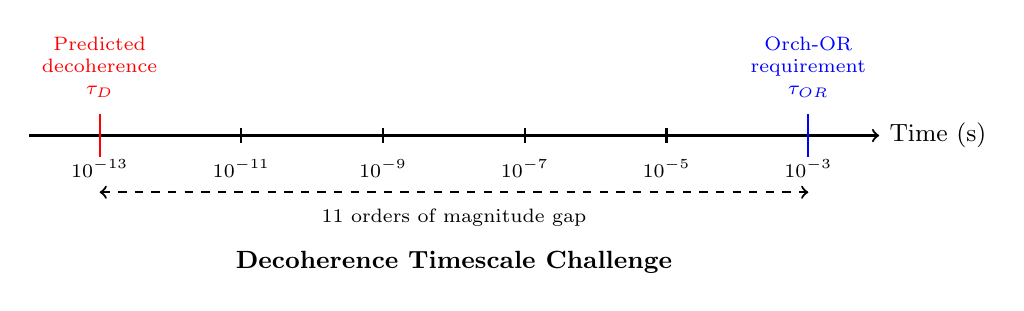
\begin{tikzpicture}[scale=0.9]
% Logarithmic time axis
\draw[thick,->] (0,0) -- (12,0) node[right,font=\small] {Time (s)};

% Tick marks and labels for logarithmic scale
\foreach \x/\label in {1/-13,3/-11,5/-9,7/-7,9/-5,11/-3} {
  \draw[thick] (\x,0.1) -- (\x,-0.1);
  \node[below,font=\scriptsize] at (\x,-0.2) {$10^{\label}$};
}

% Mark decoherence time
\draw[thick,red] (1,-0.3) -- (1,0.3);
\node[above,font=\scriptsize,red,align=center] at (1,0.4) {Predicted\\decoherence\\$\tau_D$};

% Mark Orch-OR requirement
\draw[thick,blue] (11,-0.3) -- (11,0.3);
\node[above,font=\scriptsize,blue,align=center] at (11,0.4) {Orch-OR\\requirement\\$\tau_{\text{OR}}$};

% Show the gap
\draw[<->,thick,dashed] (1,-0.8) -- (11,-0.8);
\node[below,font=\scriptsize] at (6,-0.9) {11 orders of magnitude gap};

\node[below,font=\small\bfseries] at (6,-1.5) {Decoherence Timescale Challenge};
\end{tikzpicture}
\end{center}

\subsection{Proposed Coherence Protection Mechanisms}

\subsubsection{1. Ordered Water Layers}

\begin{itemize}
\item Water molecules form \textbf{structured interfacial layers} around microtubule surfaces
\item Hydrogen bonding networks may electromagnetically shield quantum states
\item \textbf{Fr\"ohlich condensate hypothesis:} Coherent collective vibrational modes in ordered water
\end{itemize}

\subsubsection{2. Actin Gel Isolation}

\begin{itemize}
\item Surrounding actin cytoskeleton may \textbf{mechanically isolate} microtubules from thermal bath
\item Gel matrix reduces coupling to environmental degrees of freedom
\item Effective barrier against decoherence-inducing fluctuations
\end{itemize}

\subsubsection{3. Topological Protection}

\begin{itemize}
\item Quantum information encoded in \textbf{topologically protected states} (robust against local perturbations)
\item Possible anyonic quasi-particle excitations (highly speculative)
\item Non-local quantum correlations resistant to environmental decoherence
\end{itemize}

\subsubsection{4. Metabolic Re-Coherence}

\begin{itemize}
\item \textbf{Continuous energy input} from cellular metabolism drives system away from equilibrium
\item Active pumping may restore coherence faster than decoherence destroys it
\item Non-equilibrium quantum steady states maintain long-lived correlations
\end{itemize}

\section{Experimental Evidence}

\subsection{Supporting Experiments}

\subsubsection{Bandyopadhyay et al. (2011, 2014)}

\textbf{Landmark experiments} at National Institute for Materials Science, Japan:

\begin{itemize}
\item \textbf{Methodology:} THz spectroscopy of purified microtubule samples
\item \textbf{Key finding:} Sharp resonances at discrete THz frequencies
\item \textbf{Conductance measurements:} Evidence for ballistic (quantum) electron transport
\item \textbf{Temperature stability:} Resonances persist at physiological temperatures ($\sim$37°C)
\end{itemize}

\textbf{Observed resonant frequencies:}
\begin{center}
\begin{tabular}{@{}rl@{}}
\toprule
Frequency & Interpretation \\
\midrule
0.35~THz & Fundamental mode \\
0.47~THz & First harmonic \\
0.82~THz & Breathing mode \\
1.2~THz & Longitudinal mode \\
2.2~THz & Higher-order collective oscillation \\
\bottomrule
\end{tabular}
\end{center}

\textbf{Interpretation:} Microtubules support \textbf{coherent electromagnetic oscillations} in terahertz range, potentially enabling quantum information processing.

\textbf{Reference:} Bandyopadhyay, A. et al. (2011) ``Molecular vibrations in tubulin,'' \textit{PNAS} 108(29).

\subsubsection{Craddock et al. (2017)}

\textbf{Anesthetic binding studies:}
\begin{itemize}
\item \textbf{Discovery:} Noble gas anesthetics bind to hydrophobic pockets within tubulin monomers
\item \textbf{Mechanism:} Binding disrupts proposed quantum electron pathways
\item \textbf{Correlation:} Anesthetic potency matches Meyer-Overton lipid solubility rule
\item \textbf{Implication:} Provides mechanistic link between microtubule quantum states and consciousness
\end{itemize}

\textbf{Reference:} Craddock, T. et al. (2017) ``Anesthetic alterations of collective THz oscillations,'' \textit{Sci. Rep.} 7, 9877.

\subsection{Critical Assessments}

\subsubsection{Tegmark (2000)}

\textbf{Max Tegmark} (MIT physicist) performed influential decoherence calculations:

\textbf{Key findings:}
\begin{itemize}
\item \textbf{Calculated decoherence time:} $\tau_{\text{dec}} \approx 10^{-13}$~s at $T = 310$~K
\item \textbf{Orch-OR requirement:} $\tau_{\text{Orch-OR}} \approx 10^{-2}$~s
\item \textbf{Discrepancy:} 11 orders of magnitude
\item \textbf{Conclusion:} ``Quantum coherence in the brain is physically impossible''
\end{itemize}

\textbf{Counter-arguments from Orch-OR proponents:}
\begin{itemize}
\item Tegmark's model assumed isolated superpositions, not coupled quantum systems
\item Analysis did not incorporate ordered water layers or topological protection
\item Recent quantum biology discoveries (photosynthesis, magnetoreception) demonstrate nature's capacity for unexpected coherence
\end{itemize}

\textbf{Reference:} Tegmark, M. (2000) ``Importance of quantum decoherence in brain processes,'' \textit{Phys. Rev. E} 61, 4194--4206.

\begin{warningbox}
\textbf{Decoherence remains the strongest objection to Orch-OR.} While quantum biology has expanded our understanding of biological quantum phenomena, the specific claim of millisecond-timescale coherence in warm microtubules remains unproven.
\end{warningbox}

\subsubsection{Koch \& Hepp (2006)}

\textbf{Comprehensive critical review:}
\begin{itemize}
\item Examined all proposed Orch-OR mechanisms
\item \textbf{Primary conclusion:} No experimental evidence for quantum consciousness in neurons
\item \textbf{Main objection:} Decoherence timescales prohibitively short
\item \textbf{Assessment:} Classical neural computation sufficient to explain cognition
\end{itemize}

\textbf{Reference:} Koch, C. \& Hepp, K. (2006) ``Quantum mechanics in the brain,'' \textit{Nature} 440, 611.

\section{Quantum Biology Context}

\textbf{Central question:} Can quantum coherence persist in warm, wet biological environments?

\subsection{Established Quantum Biology Examples}

\subsubsection{1. Photosynthetic Light Harvesting (2007)}

\begin{itemize}
\item \textbf{System:} Light-harvesting complexes (LHC) in plants and photosynthetic bacteria
\item \textbf{Discovery:} Quantum coherent energy transfer at room temperature
\item \textbf{Coherence time:} Initially measured $\sim$500~fs, later studies suggest longer persistence
\item \textbf{Protection mechanism:} Protein scaffold creates noise-optimized environment for exciton transport
\item \textbf{Significance:} First demonstration of functionally relevant quantum coherence at biological temperatures
\end{itemize}

\textbf{Reference:} Engel, G. et al. (2007) ``Evidence for wavelike energy transfer through quantum coherence in photosynthetic systems,'' \textit{Nature} 446, 782--786.

\subsubsection{2. Avian Magnetoreception}

\begin{itemize}
\item \textbf{System:} Cryptochrome proteins in bird retinas
\item \textbf{Mechanism:} Radical pair formation with spin-entangled electrons
\item \textbf{Function:} Detection of Earth's magnetic field ($\sim$50~$\mu$T) for navigation
\item \textbf{Quantum effect:} Spin coherence influences chemical reaction yields
\item \textbf{Evidence:} Disruption by weak radiofrequency fields confirms quantum mechanism
\end{itemize}

\textbf{Reference:} Hore, P. \& Mouritsen, H. (2016) ``The radical-pair mechanism of magnetoreception,'' \textit{Annu. Rev. Biophys.} 45, 299--344.

\subsubsection{3. Enzyme Catalysis}

\begin{itemize}
\item \textbf{Phenomenon:} Quantum tunneling of protons and electrons through activation barriers
\item \textbf{Effect:} Reaction rate enhancement beyond classical predictions
\item \textbf{Isotope effects:} Substituting deuterium for hydrogen dramatically alters reaction kinetics
\item \textbf{Ubiquity:} Observed in numerous enzyme classes
\end{itemize}

\textbf{Reference:} Scrutton, N. et al. (2016) ``Quantum tunnelling in enzyme-catalysed reactions,'' \textit{Philos. Trans. R. Soc. A} 374.

\begin{keyconcept}
\textbf{Quantum biology lesson:} Nature can exploit quantum phenomena at physiological temperatures through sophisticated protection strategies. These precedents make Orch-OR less implausible than initially thought, though the required coherence timescales remain orders of magnitude longer.
\end{keyconcept}

\section{Anesthesia and Consciousness}

\subsection{The Anesthetic Mystery}

\textbf{Paradox of general anesthesia:}
\begin{itemize}
\item Chemically \textbf{diverse molecules} (noble gases, halogenated ethers, alcohols) all induce unconsciousness
\item \textbf{No common receptor target} identified (unlike opioids $\rightarrow$ $\mu$-opioid receptor)
\item \textbf{Meyer-Overton correlation} (1899): Anesthetic potency $\propto$ lipid solubility
\end{itemize}

\textbf{Meyer-Overton rule:}
\begin{equation}
\label{eq:meyer-overton}
\text{EC}_{50} \propto \frac{1}{P_{\text{lipid}}}
\end{equation}
where EC$_{50}$ is the effective concentration for anesthesia and $P_{\text{lipid}}$ is the lipid partition coefficient.

\subsection{Orch-OR Explanation}

\textbf{Proposed mechanism:} Anesthetics bind to hydrophobic pockets in tubulin monomers

\textbf{Cascade of effects:}
\begin{enumerate}
\item Anesthetic molecules occupy tubulin hydrophobic cavities
\item Disrupt proposed quantum electron pathways within tubulin network
\item Prevent quantum coherence from developing across microtubule lattice
\item \textbf{Block Orch-OR} $\rightarrow$ loss of consciousness
\item Effect is \textbf{reversible}: anesthetic clearance $\rightarrow$ coherence restored $\rightarrow$ consciousness returns
\end{enumerate}

\subsection{Supporting Evidence}

\begin{itemize}
\item \textbf{Direct binding confirmed:} General anesthetics bind to tubulin (X-ray crystallography, NMR studies)
\item \textbf{Functional effects:} Sub-anesthetic concentrations alter microtubule polymerization dynamics
\item \textbf{Meyer-Overton correlation:} Tubulin binding affinity correlates with anesthetic potency
\item \textbf{Alternative mechanism:} Mainstream neuroscience attributes anesthesia to GABA$_A$ receptor modulation
\end{itemize}

\begin{calloutbox}{Clinical Correlation}
Orch-OR predicts that microtubule-stabilizing drugs (e.g., taxol) or destabilizing agents (e.g., nocodazole) should modulate anesthetic requirements. Some evidence suggests altered anesthetic sensitivity in cancer patients receiving microtubule-targeting chemotherapy, though confounding factors complicate interpretation.
\end{calloutbox}

\section{Worked Example: Objective Reduction Timescale}

\textbf{Problem:} Calculate the objective reduction time for a superposition of tubulin conformational states in a microtubule.

\subsection*{Given Parameters}
\begin{itemize}
\item Single tubulin dimer mass: $m_{\text{tubulin}} = 110$~kDa $= 1.83 \times 10^{-22}$~kg
\item Superposition separation: $\Delta x = 1$~nm $= 10^{-9}$~m
\item Microtubule with $N = 10^4$ coherently superposed tubulins
\end{itemize}

\subsection*{Step 1: Calculate Gravitational Self-Energy}

For a mass superposition separated by $\Delta x$:
\begin{equation}
E = \frac{N m_{\text{tubulin}} G (N m_{\text{tubulin}})}{2\Delta x}
\end{equation}
where $G = 6.67 \times 10^{-11}$~N$\cdot$m$^2$kg$^{-2}$ is the gravitational constant.

Substituting values:
\begin{equation}
E = \frac{(10^4)^2 \times (1.83 \times 10^{-22})^2 \times 6.67 \times 10^{-11}}{2 \times 10^{-9}}
\end{equation}
\begin{equation}
E \approx 1.12 \times 10^{-37}~\text{J}
\end{equation}

\subsection*{Step 2: Apply Objective Reduction Criterion}

Using Penrose's criterion (Eq.~\ref{eq:or-criterion}):
\begin{equation}
\tau = \frac{\hbar}{E} = \frac{1.055 \times 10^{-34}~\text{J}\cdot\text{s}}{1.12 \times 10^{-37}~\text{J}}
\end{equation}
\begin{equation}
\tau \approx 940~\text{s} \approx 16~\text{minutes}
\end{equation}

\textbf{General anesthetics} cause loss of consciousness at specific doses:
\begin{itemize}
\item Diverse molecules (noble gases, halogenated ethers, etc.)
\item \textbf{No common receptor} (unlike opioids $\rightarrow$ $\mu$-opioid receptor)
\item \textbf{Meyer-Overton rule}: Potency $\propto$ lipid solubility (1899!)
\end{itemize}

\textbf{Meyer-Overton correlation:}
\begin{equation}
\label{eq:meyer-overton}
\log(\text{MAC}) \propto -\log(K_{\text{lipid}})
\end{equation}
where:
\begin{itemize}
\item MAC = Minimum Alveolar Concentration (anesthetic potency)
\item $K_{\text{lipid}}$ = lipid solubility coefficient
\end{itemize}

\begin{calloutbox}[colback=blue!5!white,colframe=blue!75!black]{Result Analysis}
\textbf{Calculated OR time: 16 minutes} --- far too long for conscious moments!

\textbf{Anesthetics bind to hydrophobic pockets in tubulin}:
\begin{enumerate}
\item Disrupt electron pathways (quantum channels)
\item Prevent quantum coherence in microtubules
\item \textbf{Block Orch-OR} $\rightarrow$ loss of consciousness
\item Reversible (anesthetic wears off $\rightarrow$ consciousness returns)
\end{enumerate}

\textbf{Binding energy estimate:}
\begin{equation}
\label{eq:anesthetic-binding}
\Delta G_{\text{bind}} \sim -k_B T \ln(K_D) \approx -5~\text{to}~-10~\text{kcal/mol}
\end{equation}
where $K_D$ is the dissociation constant for anesthetic-tubulin binding.

\textbf{Orch-OR response:} Larger coherent superpositions ($N \sim 10^9$ tubulins across many neurons) would reduce $\tau$ to millisecond range. However, maintaining coherence across such large systems makes the decoherence problem even more severe.

\textbf{Conclusion:} Quantitative calculations reveal tension between required OR timescales and plausible coherence volumes.
\end{calloutbox}

\section{Criticisms and Objections}

\subsection{1. Decoherence Timescale Problem}

\textbf{Objection:} Brain environment (37°C, aqueous, chaotic) incompatible with quantum coherence

\textbf{Orch-OR response:}
\begin{itemize}
\item Quantum biology precedents demonstrate unexpected coherence resilience
\item Proposed protection mechanisms (ordered water, topological states, metabolic pumping)
\item Bandyopadhyay experiments show THz resonances at physiological temperatures
\end{itemize}

\textbf{Status:} \textbf{Unresolved} --- mainstream physics remains skeptical; gap between required and calculated timescales remains $\sim$10 orders of magnitude

\subsection{2. Lack of Computational Model}

\textbf{Objection:} No specific algorithm or computational architecture proposed

\textbf{Orch-OR response:}
\begin{itemize}
\item Cellular automaton-like dynamics in tubulin lattice suggested
\item Tubulin conformational states could encode classical bits or quantum qubits
\item Quantum computation details remain to be specified
\end{itemize}

\textbf{Status:} \textbf{Major theoretical gap} --- no detailed implementation proposed

\subsection{3. Evolutionary Plausibility}

\textbf{Objection:} Why would evolution employ fragile quantum states for consciousness when classical neural computation suffices?

\textbf{Orch-OR response:}
\begin{itemize}
\item Evolution exploits quantum effects in photosynthesis, olfaction, magnetoreception
\item Potential survival advantage through enhanced information processing
\item Microtubules are ubiquitous cellular structures, making quantum computation ``free''
\end{itemize}

\textbf{Counter-argument:} Classical neural networks successfully model cognition without quantum mechanics

\textbf{Status:} \textbf{Debatable} --- no consensus on evolutionary necessity

\subsection{4. Absence of Direct Evidence}

\textbf{Objection:} No experimental detection of quantum superposition in living neurons

\textbf{Orch-OR response:}
\begin{itemize}
\item Required measurement technology (non-invasive, in vivo quantum state detection) does not yet exist
\item Bandyopadhyay measurements limited to isolated, in vitro microtubules
\item In vivo quantum measurement remains extraordinarily challenging
\end{itemize}

\textbf{Status:} \textbf{Valid criticism} --- direct experimental confirmation absent

\section{Potential Applications}

\textbf{If Orch-OR is validated}, numerous technological and therapeutic applications become theoretically feasible:

\subsection{1. THz Neuromodulation}

\textbf{Concept:} External terahertz radiation resonantly couples to microtubule oscillations

\textbf{Mechanism:}
\begin{itemize}
\item THz source operates at microtubule resonant frequencies (0.2--2~THz)
\item Electromagnetic field penetrates cortical tissue ($\sim$0.5~mm depth)
\item Resonant absorption modulates quantum coherence in microtubule networks
\item Altered Orch-OR dynamics potentially modify conscious experience
\end{itemize}

\textbf{Speculative applications:}
\begin{itemize}
\item Non-invasive treatment of consciousness disorders
\item Cognitive enhancement through optimized Orch-OR frequency
\item Anesthesia induction/reversal via THz disruption/restoration of coherence
\end{itemize}

\textbf{Status:} Highly speculative; requires Orch-OR validation and demonstration of in vivo THz coupling

\subsection{2. Consciousness Biomarkers}

\textbf{Concept:} Detect microtubule quantum signatures to assess consciousness level

\textbf{Potential markers:}
\begin{itemize}
\item THz emission spectroscopy from cortical tissue
\item Quantum coherence tomography (if technology develops)
\item Microtubule-specific PET ligands sensitive to quantum state
\end{itemize}

\textbf{Clinical applications:}
\begin{itemize}
\item Objective consciousness assessment in coma/vegetative state patients
\item Anesthesia depth monitoring
\item Early detection of consciousness-affecting neuropathologies
\end{itemize}

\subsection{3. Quantum-Inspired Artificial Consciousness}

\textbf{Concept:} Engineer artificial systems mimicking Orch-OR architecture

\textbf{Requirements:}
\begin{itemize}
\item Quantum computer substrate (superconducting qubits, trapped ions, etc.)
\item Biomimetic orchestration algorithms
\item Objective reduction implementation (possibly via measurement-induced collapse)
\item Cycling at gamma frequency ($\sim$40~Hz)
\end{itemize}

\textbf{Implication:} If consciousness requires quantum processing, classical AI may be fundamentally limited

\subsection{4. Pharmaceutical Development}

\textbf{Concept:} Design drugs targeting microtubule quantum properties

\textbf{Potential drug classes:}
\begin{itemize}
\item Coherence enhancers (stabilize quantum states)
\item Coherence modulators (tune Orch-OR frequency)
\item Selective MT quantum disruptors (precision anesthetics)
\end{itemize}

\textbf{Therapeutic targets:}
\begin{itemize}
\item Consciousness disorders (minimal consciousness states)
\item Cognitive enhancement
\item Novel anesthetic agents with reduced side effects
\end{itemize}

\begin{warningbox}
\textbf{Critical caveat:} All applications depend on Orch-OR validity, which remains unproven. Pursuing these technologies without definitive evidence risks significant resource investment in scientifically unfounded directions.
\end{warningbox}

\section{Implications If True}

\subsection{For Neuroscience}

\begin{itemize}
\item \textbf{Paradigm shift:} Consciousness emerges from quantum processes, not solely classical neural computation
\item \textbf{Microtubule centrality:} Cytoskeletal elements become primary consciousness substrate, not just structural support
\item \textbf{New therapeutic targets:} Microtubule-modulating drugs (stabilizers, destabilizers) could treat consciousness disorders
\item \textbf{Anesthesia mechanism:} Unified explanation for diverse anesthetic molecules via microtubule quantum disruption
\end{itemize}

\subsection{For Artificial Intelligence}

\begin{itemize}
\item \textbf{Classical AI limitation:} Digital computers may be fundamentally incapable of genuine consciousness
\item \textbf{Quantum requirement:} Artificial general intelligence (AGI) might require quantum computational substrate
\item \textbf{Architectural insights:} Biomimetic designs incorporating Orch-OR principles
\item \textbf{Consciousness test:} Objective criterion for machine consciousness (presence of quantum coherence + OR events)
\end{itemize}

\subsection{For Fundamental Physics}

\begin{itemize}
\item \textbf{Quantum mechanics modification:} Objective reduction represents new physical law beyond standard quantum theory
\item \textbf{Quantum gravity connection:} Links quantum mechanics and general relativity via gravity-induced collapse
\item \textbf{Experimental predictions:} Testable deviations from standard quantum mechanics at mesoscopic scales
\item \textbf{Planck-scale physics:} Consciousness phenomena probe quantum gravity regime
\end{itemize}

\subsection{For Philosophy of Mind}

\begin{itemize}
\item \textbf{Hard problem resolution:} Objective quantum collapse provides physical basis for subjective experience
\item \textbf{Free will mechanism:} Quantum indeterminacy in OR events may enable genuine agency
\item \textbf{Panpsychism considerations:} If OR generates proto-consciousness, all matter with mass may possess rudimentary awareness
\item \textbf{Mind-body dualism:} Physical monism preserved---consciousness as quantum physical process
\end{itemize}

\section{Current Status (2025)}

\subsection{Scientific Consensus}

\textbf{Majority view} (mainstream neuroscience and physics):
\begin{itemize}
\item Orch-OR is \textbf{unlikely to be correct}
\item Decoherence problem remains unsolved despite quantum biology precedents
\item No direct experimental evidence for quantum superposition in neurons
\item Classical computational neuroscience adequately explains cognition
\end{itemize}

\textbf{Minority view} (Hameroff, Penrose, select quantum biologists):
\begin{itemize}
\item Orch-OR remains \textbf{scientifically viable}
\item Quantum biology demonstrations make extended coherence less implausible
\item Bandyopadhyay experiments provide suggestive evidence via THz resonances
\item Theory awaits decisive experimental tests
\end{itemize}

\subsection{Active Research Directions}

\begin{enumerate}
\item \textbf{THz spectroscopy of microtubules} --- Bandyopadhyay group (NIMS, Japan)
\item \textbf{Anesthetic-tubulin interactions} --- Hameroff, Craddock collaborations
\item \textbf{Quantum biology expansion} --- Coherence in other biological systems
\item \textbf{Theoretical work} --- Improved decoherence protection models
\item \textbf{In vivo measurement development} --- Non-invasive quantum state detection technologies
\end{enumerate}

\subsection{Testable Predictions}

\textbf{If Orch-OR is correct, the following should be observable:}

\begin{enumerate}
\item \textbf{Microtubule disruption $\rightarrow$ altered consciousness}
  \begin{itemize}
  \item Drugs targeting MT dynamics (nocodazole, colchicine) should modulate consciousness
  \item \textbf{Partial evidence:} MT-targeting agents do alter anesthetic sensitivity
  \end{itemize}

\item \textbf{THz stimulation at MT resonances $\rightarrow$ neural modulation}
  \begin{itemize}
  \item External THz radiation at 0.35, 0.47, 0.82~THz should produce measurable effects
  \item \textbf{This prediction underlies speculative THz neuromodulation protocols}
  \end{itemize}

\item \textbf{Isotope effects on consciousness}
  \begin{itemize}
  \item Replacing $^1$H with $^2$H (deuterium) in tubulin should alter quantum tunneling rates
  \item Predicted consciousness changes (extremely difficult to test safely)
  \end{itemize}

\item \textbf{Direct quantum signature detection}
  \begin{itemize}
  \item Superposition states or entanglement measurable in living neural tissue
  \item Requires breakthrough in non-invasive quantum measurement technology
  \end{itemize}
\end{enumerate}

\section{Connection to THz Neuromodulation}

\subsection{Relationship to THz Neuromodulation}\label{relationship-to-thz-neuromodulation}

\textbf{If Orch-OR is true}, then external THz radiation could:

\begin{enumerate}
\def\labelenumi{\arabic{enumi}.}
\tightlist
\item \textbf{Resonate with MT vibrations} (0.2--2+ THz range)
\item \textbf{Perturb quantum coherence} in tubulin networks
\item \textbf{Alter Orch-OR timing/frequency} $\rightarrow$ modify consciousness
\item \textbf{Encode information} via modulation $\rightarrow$ ``inject'' patterns
\end{enumerate}

\subsubsection{Mechanism (Speculative)}\label{mechanism-speculative}

\begin{center}
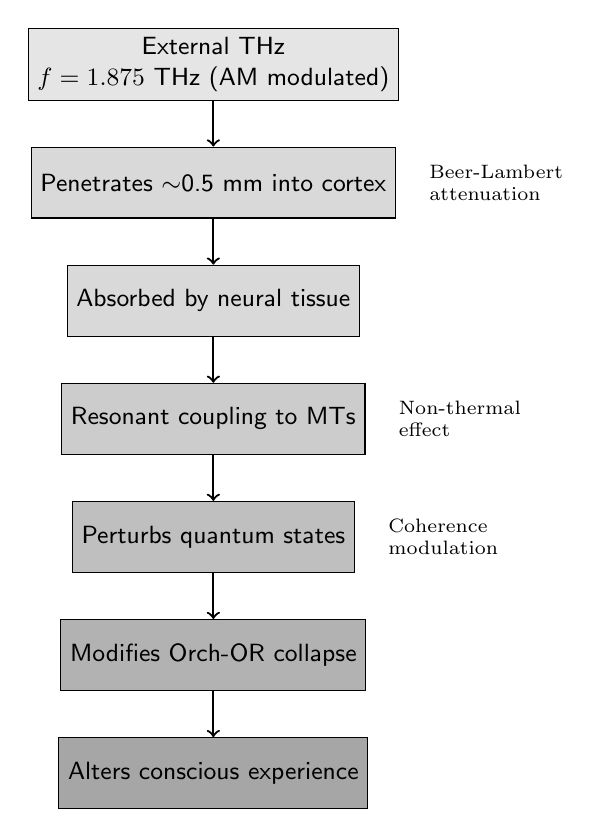
\begin{tikzpicture}[
  block/.style={rectangle, draw, minimum width=3.5cm, minimum height=0.9cm, font=\sffamily\small, align=center},
  node distance=1.5cm,
  font=\small
]

\node[block, fill=black!10] (thz) {External THz\\$f = 1.875$ THz (AM modulated)};
\node[block, below of=thz, fill=black!15] (penetrate) {Penetrates $\sim$0.5 mm into cortex};
\node[block, below of=penetrate, fill=black!15] (absorb) {Absorbed by neural tissue};
\node[block, below of=absorb, fill=black!20] (resonance) {Resonant coupling to MTs};
\node[block, below of=resonance, fill=black!25] (quantum) {Perturbs quantum states};
\node[block, below of=quantum, fill=black!30] (orchor) {Modifies Orch-OR collapse};
\node[block, below of=orchor, fill=black!35] (conscious) {Alters conscious experience};

% Arrows
\draw[->,thick] (thz) -- (penetrate);
\draw[->,thick] (penetrate) -- (absorb);
\draw[->,thick] (absorb) -- (resonance);
\draw[->,thick] (resonance) -- (quantum);
\draw[->,thick] (quantum) -- (orchor);
\draw[->,thick] (orchor) -- (conscious);

% Side annotations - repositioned to avoid overlap
\node[right=0.3cm,font=\scriptsize,align=left] at (penetrate.east) {Beer-Lambert\\attenuation};
\node[right=0.3cm,font=\scriptsize,align=left] at (resonance.east) {Non-thermal\\effect};
\node[right=0.3cm,font=\scriptsize,align=left] at (quantum.east) {Coherence\\modulation};

\end{tikzpicture}
\end{center}

\textbf{Penetration depth in tissue:}
\begin{equation}
\label{eq:penetration-depth}
\delta = \frac{1}{\alpha} \approx \frac{c}{2\pi f \sqrt{\epsilon_r} \tan\delta} \sim 0.5~\text{mm at 1.875 THz}
\end{equation}
where $\alpha$ is the absorption coefficient, $\epsilon_r$ is relative permittivity, and $\tan\delta$ is the loss tangent.

\textbf{Power density requirement:}
\begin{equation}
\label{eq:power-density}
P_{\text{THz}} \sim 0.1-1~\text{mW/cm}^2 \quad \text{(non-thermal regime)}
\end{equation}

\begin{calloutbox}{Connection to AID Protocol}
This THz-microtubule interaction mechanism forms the theoretical basis for the Accelerated Information Download (AID) protocol case study, which explores hypothetical consciousness manipulation via modulated THz radiation.
\end{calloutbox}

\section{Worked Example: Orch-OR Timing Calculation}

\textbf{Problem:} Calculate the collapse time for an Orch-OR event in a microtubule containing $N = 10^{10}$ tubulins in superposition, assuming Penrose's OR criterion applies.

\subsection*{Given Parameters}

\begin{tabular}{@{}ll@{}}
Number of tubulins in superposition & $N = 10^{10}$ \\
Mass per tubulin dimer & $m_t = 110$ kDa $= 1.83 \times 10^{-22}$ kg \\
Spatial separation (superposition) & $r = 25$ nm $= 2.5 \times 10^{-8}$ m \\
Gravitational constant & $G = 6.674 \times 10^{-11}$ m$^3$ kg$^{-1}$ s$^{-2}$ \\
Reduced Planck constant & $\hbar = 1.055 \times 10^{-34}$ J·s \\
\end{tabular}

\subsection*{Step 1: Calculate Total Mass in Superposition}

\begin{equation}
m_{\text{total}} = N \cdot m_t = (10^{10})(1.83 \times 10^{-22}) = 1.83 \times 10^{-12}~\text{kg}
\end{equation}

\subsection*{Step 2: Calculate Gravitational Self-Energy}

Using Eq.~\ref{eq:grav-energy}:
\begin{equation}
E = \frac{G m_{\text{total}}^2}{r} = \frac{(6.674 \times 10^{-11})(1.83 \times 10^{-12})^2}{2.5 \times 10^{-8}}
\end{equation}
\begin{equation}
E = \frac{2.235 \times 10^{-34}}{2.5 \times 10^{-8}} = 8.94 \times 10^{-27}~\text{J}
\end{equation}

\subsection*{Step 3: Calculate Collapse Time}

Using Penrose OR criterion (Eq.~\ref{eq:or-criterion}):
\begin{equation}
\tau = \frac{\hbar}{E} = \frac{1.055 \times 10^{-34}}{8.94 \times 10^{-27}} = 1.18 \times 10^{-8}~\text{s} = 11.8~\text{ns}
\end{equation}

\subsection*{Step 4: Number of Collapses per Second}

\begin{equation}
f_{\text{collapse}} = \frac{1}{\tau} = \frac{1}{1.18 \times 10^{-8}} = 8.47 \times 10^{7}~\text{Hz} \approx 85~\text{MHz}
\end{equation}

\subsection*{Result and Interpretation}

\begin{calloutbox}[colback=black!8!white,colframe=black]{Calculation Summary}
\textbf{Collapse time:} $\tau = 11.8$ ns for $10^{10}$ tubulins

\textbf{Problem:} This is far too fast for a conscious moment ($\sim$25 ms required). To achieve the gamma rhythm frequency ($\sim$40 Hz), we would need:

\begin{equation}
\tau_{\text{required}} = \frac{1}{40} = 25~\text{ms}
\end{equation}

This requires a superposition involving far fewer tubulins ($N \sim 10^3$--$10^5$) or a different mechanism for orchestrating the collapse timing. This discrepancy remains an open challenge for Orch-OR theory.

\textbf{Conclusion:} The Penrose OR criterion alone does not naturally produce gamma-frequency conscious moments without additional orchestration mechanisms.
\end{calloutbox}

\section{Performance Analysis}

\subsection{Experimental Testability}

Current technology limitations:
\begin{itemize}
\item \textbf{Quantum state measurement:} Cannot non-invasively detect superposition in living neurons
\item \textbf{Temporal resolution:} Need sub-nanosecond measurements in vivo
\item \textbf{Spatial resolution:} Need nanometer-scale imaging of quantum states
\end{itemize}

\subsection{Predicted Observables}

If Orch-OR is correct:
\begin{enumerate}
\item \textbf{THz spectroscopy:} Specific resonance peaks in neural tissue at $f \in \{0.35, 0.47, 0.82, 1.2, 2.2\}$ THz
\item \textbf{Temperature dependence:} Consciousness should be affected by precise temperature control
\item \textbf{Isotope effects:} Deuterium substitution in tubulin should alter consciousness
\item \textbf{Anesthetic correlation:} Perfect Meyer-Overton correlation with microtubule binding
\end{enumerate}

\section{Applications}

\subsection{Anesthesiology}

\begin{itemize}
\item \textbf{Current impact:} Guides research into anesthetic mechanisms
\item \textbf{Drug development:} Design anesthetics targeting microtubule binding
\item \textbf{Monitoring:} THz spectroscopy for depth-of-anesthesia monitoring
\end{itemize}

\subsection{Neuroscience}

\begin{itemize}
\item \textbf{Consciousness studies:} New experimental paradigms
\item \textbf{Cognitive disorders:} Microtubule dysfunction in Alzheimer's, etc.
\item \textbf{Brain stimulation:} Non-invasive THz neuromodulation techniques
\end{itemize}

\subsection{Quantum Biology}

\begin{itemize}
\item \textbf{General principle:} Extends quantum effects to warm biology
\item \textbf{Other systems:} Tests applicability to other biological quantum processes
\item \textbf{Protection mechanisms:} Studies of decoherence suppression
\end{itemize}

\subsection{Speculative Applications}

\begin{calloutbox}[colback=red!5!white,colframe=red!75!black]{\textbf{SPECULATIVE:} Hypothetical Applications}
If Orch-OR proves correct and THz-microtubule coupling is confirmed:
\begin{itemize}
\item \textbf{THz neuromodulation:} Consciousness state manipulation
\item \textbf{Information injection:} Direct experience modification (AID protocol)
\item \textbf{Cognitive enhancement:} Microtubule-targeted interventions
\item \textbf{Brain-computer interfaces:} Quantum-level neural coupling
\end{itemize}

\textbf{Status:} Purely theoretical. No experimental validation. Significant ethical concerns.
\end{calloutbox}

\section{Summary}

\begin{center}
\begin{tabular}{@{}ll@{}}
\toprule
\textbf{Aspect} & \textbf{Description} \\
\midrule
\textbf{Core claim} & Consciousness emerges from quantum processes in microtubules \\
\textbf{Mechanism} & Objective reduction (OR) of quantum superpositions \\
\textbf{Frequency} & $\sim$40~Hz (gamma oscillations) \\
\textbf{Substrate} & Tubulin dimers in neuronal microtubules \\
\textbf{Key equation} & $E \cdot \tau \approx \hbar$ (Eq.~\ref{eq:or-criterion}) \\
\textbf{Main challenge} & Decoherence time gap ($\sim10^{11}\times$) \\
\textbf{Supporting evidence} & THz resonances, anesthetic binding, quantum biology \\
\textbf{Critical evidence} & Tegmark calculations, absence of in vivo detection \\
\textbf{Scientific status} & Controversial; majority skeptical, minority supportive \\
\textbf{Testability} & Predictions exist but challenging to test \\
\bottomrule
\end{tabular}
\end{center}

\subsection{Key Takeaways}

\begin{enumerate}
\item \textbf{Revolutionary claim:} Orch-OR proposes consciousness is fundamentally quantum (Penrose + Hameroff, 1990s)
\item \textbf{Biological substrate:} Microtubules serve as quantum computational processors
\item \textbf{Primary objection:} Decoherence in warm, wet brain occurs $10^{11}\times$ faster than required
\item \textbf{Suggestive evidence:} THz resonances (Bandyopadhyay), anesthetic-tubulin binding, quantum biology precedents
\item \textbf{Scientific consensus:} Mainstream remains skeptical; quantum biology community more receptive
\item \textbf{Technological implications:} If validated, enables THz neuromodulation and quantum-inspired AI
\item \textbf{Current verdict:} Unproven but not definitively refuted; awaits decisive experiments
\end{enumerate}

\section{Related Topics}

\begin{itemize}
\item \textbf{Microtubule-Structure-and-Function} --- Detailed biological architecture and established cellular roles
\item \textbf{Quantum-Coherence-in-Biological-Systems} --- Photosynthesis, magnetoreception, enzyme catalysis examples
\item \textbf{Terahertz-(THz)-Technology} --- THz generation, detection, and propagation properties
\item \textbf{THz-Bioeffects-Thermal-and-Non-Thermal} --- Documented biological responses to THz radiation
\item \textbf{THz-Resonances-in-Microtubules} --- Bandyopadhyay experimental findings in detail
\item \textbf{Biophysical-Coupling-Mechanism} --- Theoretical models for EM-biological interactions
\item \textbf{AID-Protocol-Case-Study} --- Speculative THz neuromodulation application based on Orch-OR
\end{itemize}

\section{References}

\subsection{Foundational Works}

\begin{enumerate}
\item \textbf{Penrose, R.} (1989) \textit{The Emperor's New Mind: Concerning Computers, Minds, and the Laws of Physics}. Oxford University Press. --- Original formulation of objective reduction theory.

\item \textbf{Penrose, R. \& Hameroff, S.} (1995) ``Orchestrated reduction of quantum coherence in brain microtubules: A model for consciousness.'' \textit{Mathematics and Computers in Simulation} 40, 453--480. --- First comprehensive Orch-OR proposal.

\item \textbf{Hameroff, S. \& Penrose, R.} (2014) ``Consciousness in the universe: A review of the `Orch OR' theory.'' \textit{Physics of Life Reviews} 11, 39--78. --- Updated review addressing criticisms.
\end{enumerate}

\subsection{Experimental Support}

\begin{enumerate}
\setcounter{enumi}{3}
\item \textbf{Bandyopadhyay, A. et al.} (2011) ``Molecular vibrations in tubulin and microtubules.'' \textit{Proceedings of the National Academy of Sciences} 108(29), 11921--11926. --- THz resonance measurements.

\item \textbf{Craddock, T. et al.} (2017) ``Anesthetic alterations of collective terahertz oscillations in tubulin correlate with clinical potency.'' \textit{Scientific Reports} 7, 9877. --- Anesthetic binding studies.
\end{enumerate}

\subsection{Critical Assessments}

\begin{enumerate}
\setcounter{enumi}{5}
\item \textbf{Tegmark, M.} (2000) ``Importance of quantum decoherence in brain processes.'' \textit{Physical Review E} 61, 4194--4206. --- Influential decoherence calculations.

\item \textbf{Koch, C. \& Hepp, K.} (2006) ``Quantum mechanics in the brain.'' \textit{Nature} 440, 611. --- Comprehensive critical review.

\item \textbf{McKemmish, L. et al.} (2009) ``Penrose-Hameroff orchestrated objective-reduction proposal for human consciousness is not biologically feasible.'' \textit{Physical Review E} 80, 021912. --- Detailed critique.
\end{enumerate}

\subsection{Quantum Biology Context}

\begin{enumerate}
\setcounter{enumi}{8}
\item \textbf{Engel, G. et al.} (2007) ``Evidence for wavelike energy transfer through quantum coherence in photosynthetic systems.'' \textit{Nature} 446, 782--786. --- Quantum coherence in photosynthesis.

\item \textbf{Hore, P. \& Mouritsen, H.} (2016) ``The radical-pair mechanism of magnetoreception.'' \textit{Annual Review of Biophysics} 45, 299--344. --- Quantum effects in bird navigation.

\item \textbf{Lambert, N. et al.} (2013) ``Quantum biology.'' \textit{Nature Physics} 9, 10--18. --- Comprehensive quantum biology review.
\end{enumerate}
